% !TeX spellcheck = en_US
\addsection{Combat}{\skills/attack.png}

\begin{multicols*}{2}

\hypertarget{Combat}{Combat} is resolved on the separate Combat Board.
Combat with \textbf{Neutral Units} starts when a Hero moves to an unvisited Field with a roman numeral, which signifies the \hyperlink{Difficulty}{type and number} of Neutral Units guarding that field.

Combat with \textbf{another player} can start in two ways:
\begin{itemize}
  \item You move into any Field containing one of their Heroes.
  \item You move into a Town or Settlement owned by them.
\end{itemize}
Players are able to start multiple combats during their turn.

\subsection*{\hypertarget{Combatsetup}{Combat Setup}}

% TODO info about battlefield expansion
Combat takes place on the 4 x 5 Combat board, which consists of two Backlines and two Frontlines on opposite ends, and a middle row.
Follow these steps when Combat begins against \textbf{Neutral Units}:

\begin{itemize}
  \item Choose one of the Combat Board's sides as your own.
    Place up to 5 of your Unit cards freely onto the Back- and Frontline of that side.
  \item Check the \textbf{Difficulty Table} and draw the corresponding number of Neutral Unit cards from their decks.
  \item The Neutral Units are placed differently depending on the Game Mode:
  \item In \textbf{Clash} or \textbf{Alliance} Scenarios, the enemy player sitting to your right controls the Neutral Units and decides their placement.
    \includesvg[height=10px]{\svgs/unit_ranged.svg} Units must be placed in the backline if possible.
  \item In \textbf{Campaign} or \textbf{Co-op} scenarios, Neutral Units are placed from left to right from the player's perspective.
First, place any \includesvg[height=10px]{\svgs/unit_ranged.svg} units in the Backline.
Then, place any \includesvg[height=10px]{\svgs/unit_ground.svg} or \includesvg[height=10px]{\svgs/unit_flying.svg} Units in the Frontline.
If there's not enough room to place a Unit in its correct line, place them in the other one.
Units must be placed in decreasing Initiative order.
If there's a tie, place higher tier units first.
If there's still a tie, the players decide the placement order.
\end{itemize}
Unit setup when fighting \textbf{other players}:
\begin{itemize}[wide]
  \item The attacking player places up to 5 Units on their chosen side of the Combat Board, followed by the defender.
  \item If the combat takes place in a Town with a Citadel, the defender adds the \hyperlink{Walls}{Wall, Gate and Arrow Tower} cards after placing their Units.
\end{itemize}


\vspace*{\fill}
\hspace{3.6em}
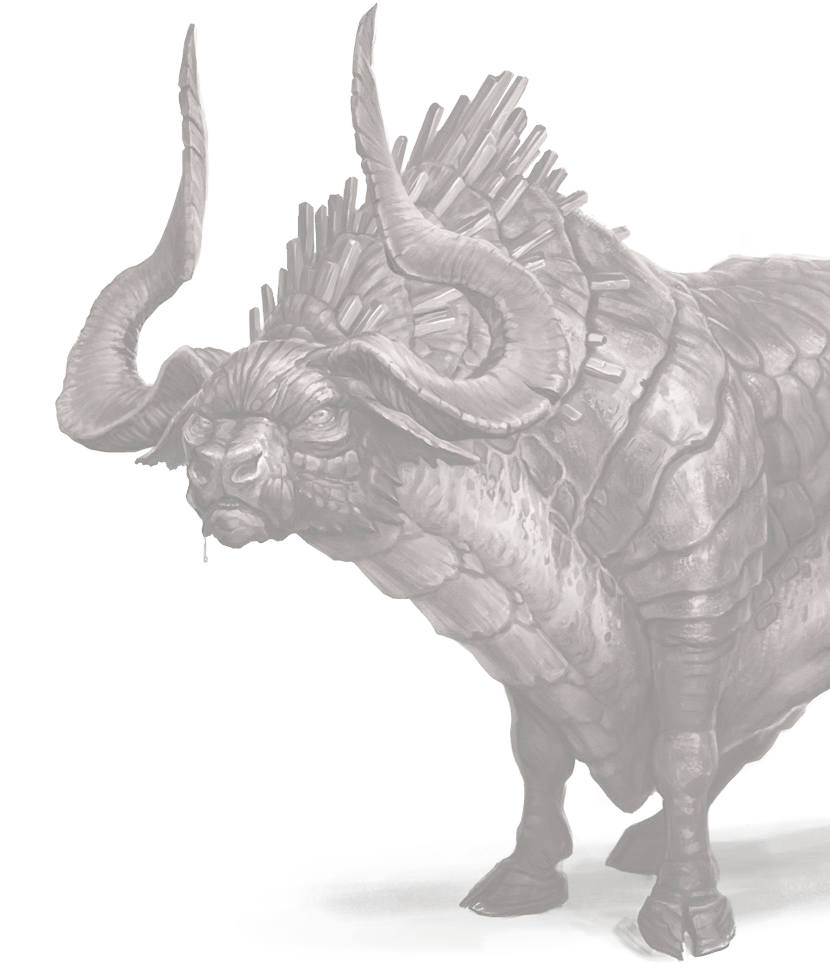
\includegraphics[width=1.05\linewidth]{\art/gorgone.png}

\subsection*{\hypertarget{Combatterminology}{Combat Terminology}}
The following terms are used in this rule book and by the Unit and other cards to describe effects and elements during combat:\par
\textbf{Attacking Playe}r – The player who started the Combat by moving their Hero.\par
\textbf{Defending Player} – The player whom Combat was started against.\par
\textbf{Activation} – A Unit activates when it is next in the Initiative order.\par
\textbf{Adjacent Unit} – A Unit is directly adjacent to another if it is one space away in a cardinal direction (nondiagonal).\par
\textbf{Combat Round} – A full cycle of all Units of each player being Activated.\par
\textbf{Combat Obstacles} – Every card placed on the Combat Board counts as a Combat Obstacle.
Obstacles block the movement of all non-flying Units.\par
\textbf{Attack Die} – A red die whose results range from -1 to +1.
Roll the die whenever a unit attacks and
add the result to the unit's attack value.\par
\textbf{\hypertarget{Retaliate}{Retaliation Attack}} – If a unit survives an attack by an adjacent Unit, it performs an attack back on that Unit.
Each Unit can perform only 1 Retaliation Attack per Combat Round.
Retaliation Attacks function identically to normal attacks, but they cannot cause another Retaliation Attack.
Mark Units which have performed a Retaliation Attack this round with a black cube.\par
\textbf{Paralysis} \includesvg[height=10px]{\svgs/paralysis.svg} – Effects which paralyze a unit place the paralysis token on them.
A paralyzed Unit \textbf{skips its next Activation} and removes the token instead.
If it is \textbf{attacked or takes any damage} before that time, \textbf{remove the paralysis token} from that unit.\par
\textbf{\hypertarget{Defend}{Defend}} \includesvg[height=10px]{\svgs/defense.svg} – When a Unit with a Defense Token is attacked, make another roll with the attack die
after the initial attack roll.
If you roll a “+1”, the defending Unit gains an extra 1 defense for this attack.
If a Unit has a defense token at the start of its activation, discard it.
The Unit cannot take another defense action during that activation.

\subsection*{\hypertarget{CombatCards}{Using Cards During Combat}}
You may only use \textbf{one Spell per Combat Round}.
Other card types can be used as many times as you want to.
Ongoing \includesvg[height=10px]{\svgs/ongoing.svg} and \includesvg[height=10px]{\svgs/activation.svg} Activate effects can be used only when Activating one of your Units and before it attacks.
Ongoing effects last until end of Combat or if the effect on the card is used up.
Instant \includesvg[height=10px]{\svgs/instant.svg} Cards may be played at any time except between rolling the Combat Die and resolving damage unless otherwise stated.
Instant Cards which increase a unit's statistics \textbf{last only for the duration of the currently activated Unit's next attack}.
\subsection*{\hypertarget{Timelimit}{Combat Time Limits}}
Combat against Neutral Units has a time limit of \textbf{one Combat Round}.
If the player cannot win the Combat before the end of the current Combat Round, they must either \hyperlink{Endcombat}{Retreat} or spend 1 MP from the Hero that started the combat in order to play another Combat Round.\par
\textbf{Note}: Combat against Azure \includesvg[height=10px]{\svgs/azure.svg} Units, other players or \hyperlink{AIrules}{AI Heroes} have no time limit.

\vspace*{\fill}
\hspace{2em}
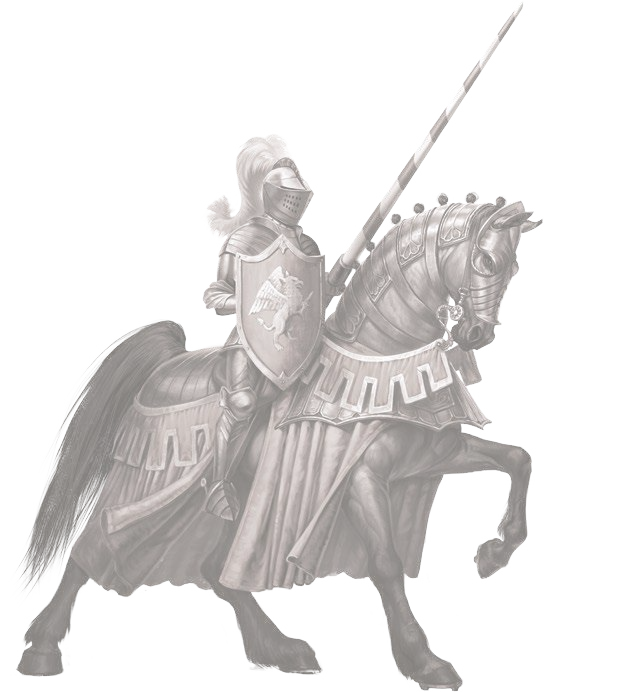
\includegraphics[width=0.9\linewidth]{\art/cavalryman.png}

\end{multicols*}

\begin{multicols}{2}

\subsection*{\hypertarget{Walls}{Defending a Town With a Citadel}}

When a Town with a Citadel is attacked, the defender adds the Wall and Gate Obstacles in any order to the Middle Row of the Combat Board after placing their Units.
The Gate Card is \textbf{not an Obstacle to the defending player}.
The Wall and Gate cards can be destroyed by any adjacent \includesvg[height=10px]{\svgs/unit_ground.svg} or \includesvg[height=10px]{\svgs/unit_flying.svg} Unit's attack.
Such attacks are always successful, do not roll the Combat Die when performing them.\par

Defending Units standing on their own side and \textbf{in the same column} as a Wall or a Gate are partially protected from \includesvg[height=10px]{\svgs/unit_ranged.svg} attacks.
If they are targeted by a \includesvg[height=10px]{\svgs/unit_ranged.svg} attack performed from the opponent's side of the Combat Board, \textbf{reduce the attack's damage by 1}.

\begin{center}
  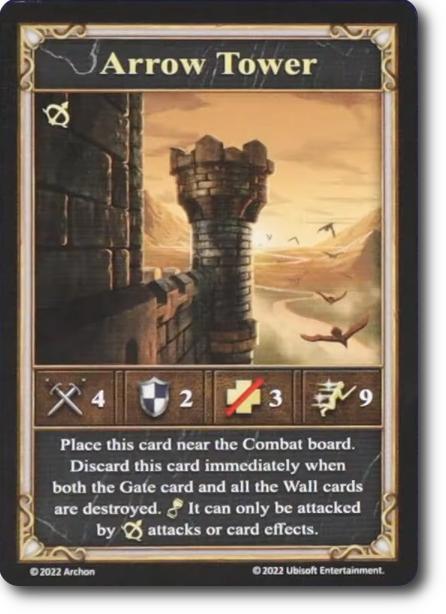
\includegraphics[width=0.6\linewidth]{\cards/arrow_tower.png}
\end{center}
The defender also gains the Arrow Tower Unit Card which is placed next to the Combat Board.

\end{multicols}

\vspace*{\fill}

\begin{figure*}[!hb]
  \mbox{}%
  \hfill%
  \begin{minipage}[t]{0.4\textwidth}
    \centering
    \shadowimage[width=\linewidth]{\examples/ranged_protected.jpg}
  \caption[halberdiers protected]{\textit{Halberdiers are behind a non-destroyed Gate, they \textbf{are protected} when attacked from spaces 1-8.}}
  \end{minipage}
  \hfill%
  \begin{minipage}[t]{0.4\textwidth}
    \centering
    \shadowimage[width=\linewidth]{\examples/ranged_unprotected.jpg}
  \caption[halberdiers unprotected]{\textit{Because Halberdiers are not behind a non-destroyed Wall, \textbf{protection doesn't work}, regardless of where the \includesvg[height=10px]{\svgs/unit_ranged.svg} attack comes from.}}
  \end{minipage}
  \hfill%
  \mbox{}%
\end{figure*}

\begin{multicols}{2}

\subsection*{Combat Round Structure}
Combat is divided into Rounds, during which all of the Units participating in that Combat \textbf{Activate once} in Initiative order.
After each Unit has activated, a new Combat Round begins.
Combat lasts until all Units on one side are eliminated, a player has to \textbf{retreat} when fighting Neutral Units, or a player \textbf{Surrenders} to another player.

Structure of a combat round:
\begin{itemize}
  \item Players Activate their Units in decreasing order of Unit \hyperlink{Initiative}{Intiative}.
  \item When a unit Activates, place a Faction Cube on it to indicate it has been Activated this Combat Round.
  \item Activated Units may move and attack according to their \hyperlink{Unittype}{type}.
  \item Instead of attacking, a Unit may \hyperlink{Defend}{defend}.
  In Neutral Combat, the Neutral Enemy units cannot defend, even when controlled by another player.
  \item Before a Unit attacks, both players may \hyperlink{CombatCards}{play cards}. Cards are resolved in the order in which players decide to play them.
  \item After a Unit's attack has been declared and all cards have been played that the players wish to play, roll the Combat Die.
    Modify the attacking Unit's attack by the die's result, then reduce it by the defending Unit's defense, and finally deal the rest as \hyperlink{HP}{damage} to the defending Unit.
  \item If the defending Unit was adjacent to the attacker, it \hyperlink{Retaliate}{retaliates} if it hasn't done so this round.
  \item Keep activating Units until they've all been activated once.
After the last Unit's activation, the combat round ends.
\end{itemize}
\subsection*{\hypertarget{Endcombat}{End Of Combat}}
Combat can end in the following ways:
\begin{itemize}
    \item All Units on one side are defeated.
    \item A player runs out of time against Neutral Units and has to \textbf{Retreat}.
    \item A player \textbf{Surrenders} when fighting another player.
\end{itemize}
In combat against \textbf{Neutral Units}, if the player defeats all opposing Units they win the combat.
If the player \hyperlink{Timelimit}{runs out of time} or all of their Units are defeated, they instead have to \textbf{Retreat}; move any surviving Units back to your Unit Deck and move the Hero that started the Combat back to the Field they last Visited.
There are no other negative consequences.
\textbf{Important exception}: If \textbf{all} of your Units from your Unit Deck were defeated during that Neutral Combat, your Main Hero must instead be moved to a friendly Town or Settlement. Secondary Heroes are removed from the game until Recruited again.\par
If you defeat all Units \textbf{during combat against another player's Main Hero}, the defeated player \textbf{loses Morale} and has to \textbf{pay the winner} 5 \includesvg[height=10px]{\svgs/gold.svg}.
Do not lose Morale or pay \includesvg[height=10px]{\svgs/gold.svg} if a \textbf{Secondary Hero} is defeated.
\textbf{In both cases}, the defeated player also \textbf{gives the winner} one of their \hyperlink{End}{faction cubes}.
Defeated Main Heroes \textbf{have to move} to a friendly Town or Settlement, while Secondary Heroes are removed from the game until Recruited again.\par
You may \textbf{Surrender} to other players by paying the other player 10 \includesvg[height=10px]{\svgs/gold.svg} when activating a Unit.
Move your Main Hero or remove your Secondary Hero from the game as if you were defeated by losing your Units.
There are no other direct consequences to Surrendering; the winner does not gain a Faction Cube.
\textbf{Note}: You cannot surrender when defending a Town.\par
When a Secondary Hero is attacked, they may also choose to be \textbf{instantly defeated} instead of fighting a Combat in order to preserve their Units.
When this happens, the attacker still receives a Faction Cube from the defeated Hero.
Defeating a Main Hero \hyperlink{End}{may eliminate} that player.\par
When Combat ends, all damage is healed from all surviving Units.
Move any player owned Units back to their Unit Deck and discard any leftover enemy Neutral Units.
After winning Combat, Heroes \textbf{must} Visit the Field where the Combat took place.

\subsection*{\hypertarget{Combatexperience}{Combat Experience}}

Winning Combat with your Main Hero usually grants them Experience.
If either the Difficulty of the Neutral Field or the Level of a defeated enemy Main Hero was equal to your Level, gain 1 \includesvg[height=10px]{\svgs/exp.svg}.
If they were higher than your Level, gain 2 \includesvg[height=10px]{\svgs/exp.svg}.
Winning a Neutral Combat which involved an Azure \includesvg[height=10px]{\svgs/azure.svg} Unit grants your Hero Level 7 immediately.
If you gain multiple Levels in this way, resolve their effects in order.\par
Secondary Heroes cannot ever gain Experience.
You also \textbf{do not gain} Experience from defeating a Secondary Hero, or if an enemy Hero Surrenders to you.
\subsection*{\hypertarget{Quick}{Quick Combat}}
If your Hero's Level is higher than a Field's Difficulty when Combat against Neutral Units would begin, \textbf{no Combat} takes place.
The player is considered to have beaten the Neutral Units by default and gains no rewards from the Combat.

\subsection*{\hypertarget{AIrules}{Player vs AI}}
These rules apply when playing a \textbf{Solo} game.
The AI Combat rules for targeting and attacking are also used when playing a \textbf{Cooperative} Scenario.\par
Solo Campaigns are played against AI Heroes who use two automated decks to play the game: the AI Deck, and the Spell Deck.
The AI Deck consists of cards that are similar in function to Abilities and Artifacts, but change depending on the game's \hyperlink{Difficulty}{Difficulty}.
The Spell Deck should be used when instructed by the cards in the AI Deck.
During combat against Neutral enemies or AI Heroes, their Units follow an automatic set of instructions.
\textbf{Initiative rules} work identically.
When an \textbf{AI hero} Activates a Unit, draw an AI card and follow its instructions as the Unit's Activation.\par
All AI controlled \includesvg[height=10px]{\svgs/unit_ground.svg} and \includesvg[height=10px]{\svgs/unit_flying.svg} Units prioritize attacking Units of the same tier.
If this is impossible, they attack the closest Unit, prioritizing the lowest tier one.
\includesvg[height=10px]{\svgs/unit_ranged.svg} Units prioritize attacking other \includesvg[height=10px]{\svgs/unit_ranged.svg} Units of the same tier, then lower tier, and finally higher tier.
If there are no \includesvg[height=10px]{\svgs/unit_ranged.svg} Units for them to target they prioritize \includesvg[height=10px]{\svgs/unit_ground.svg} and \includesvg[height=10px]{\svgs/unit_flying.svg} Units in the same tier order.
If there's more than one valid target, they attack the closest one.\par
If there's ever a tie between equally valid targets for any units, the players choose which Unit is attacked.

\textbf{AI Ueroes} always start in their Town's Field unless otherwise stated.
They have 3MP and always use them to perform the following actions in decreasing priority:
\begin{itemize}
  \item Check if a player Hero is on the same Tile as the AI.
    If they are, spend all MP to move towards them in an attempt to begin Combat.
  \item Check if there are any Mines or Settlements to Flag on the Map Tile the AI Hero is on.
    If there are any, move toward the closest one and Flag it.
  \item Otherwise, move toward the player's Town in an attempt to Flag it.
Repeat this sequence until all MP is used.
\end{itemize}

\begin{center}
  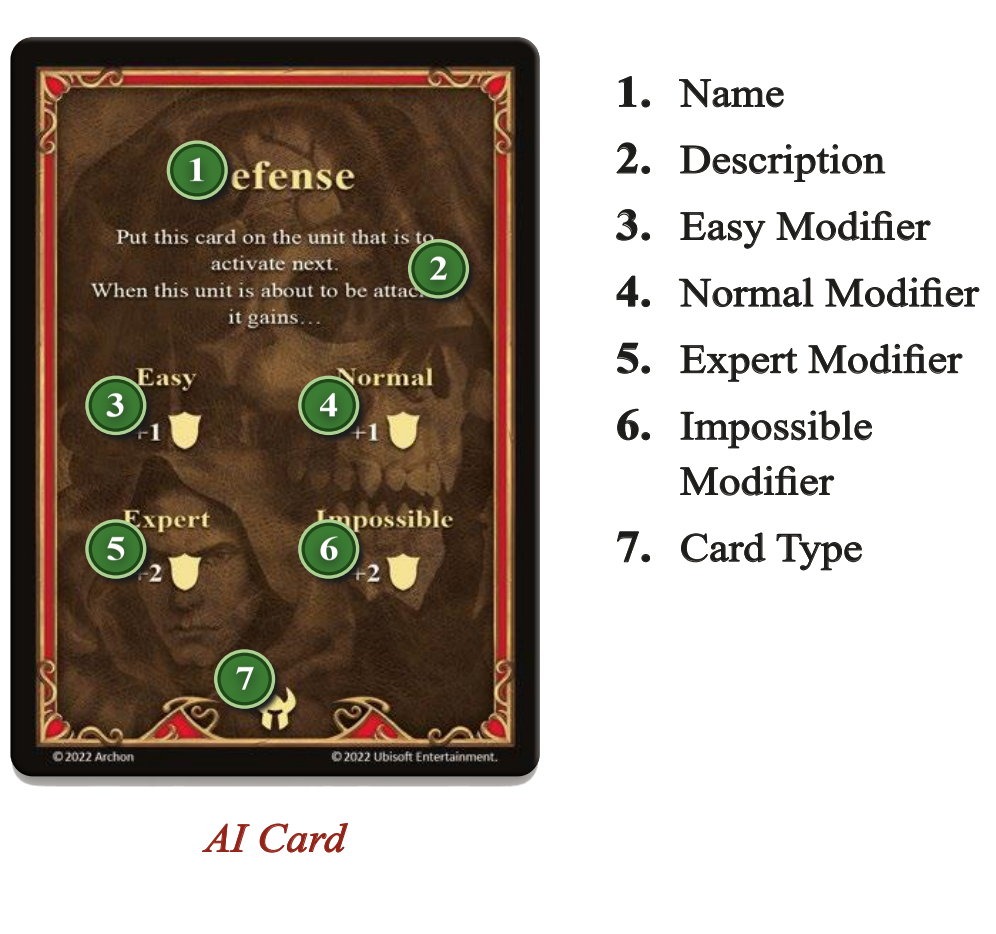
\includegraphics[width=\linewidth]{\cards/ai.png}
\end{center}

AI Heroes always \textbf{automatically win Combat} against any Neutral Units, while simultaneously \textbf{Flagging or Visiting all fields} they happen to move through.
They gain no benefits from Flagging or Visiting Fields.

AI Heroes must discover face down Map Tiles as normal by spending 1 MP before moving onto them.
The player chooses that tile's orientation.\par
AI Heroes cannot Surrender and you cannot Surrender to them;
they will always fight until they run out of Units.
Winning Combat against an AI Hero does not grant any rewards unless stated by the Scenario.
AI Heroes do not have a Town Board, Resources, or a Hero Card.
Their Units are static and defined by the Scenario's setup or other rules.\par
Any differences to the above will be described in any given Scenario's own rules.


\end{multicols}

\vspace*{\fill}
\begin{scaledfigure}[blanker]
  \centering
  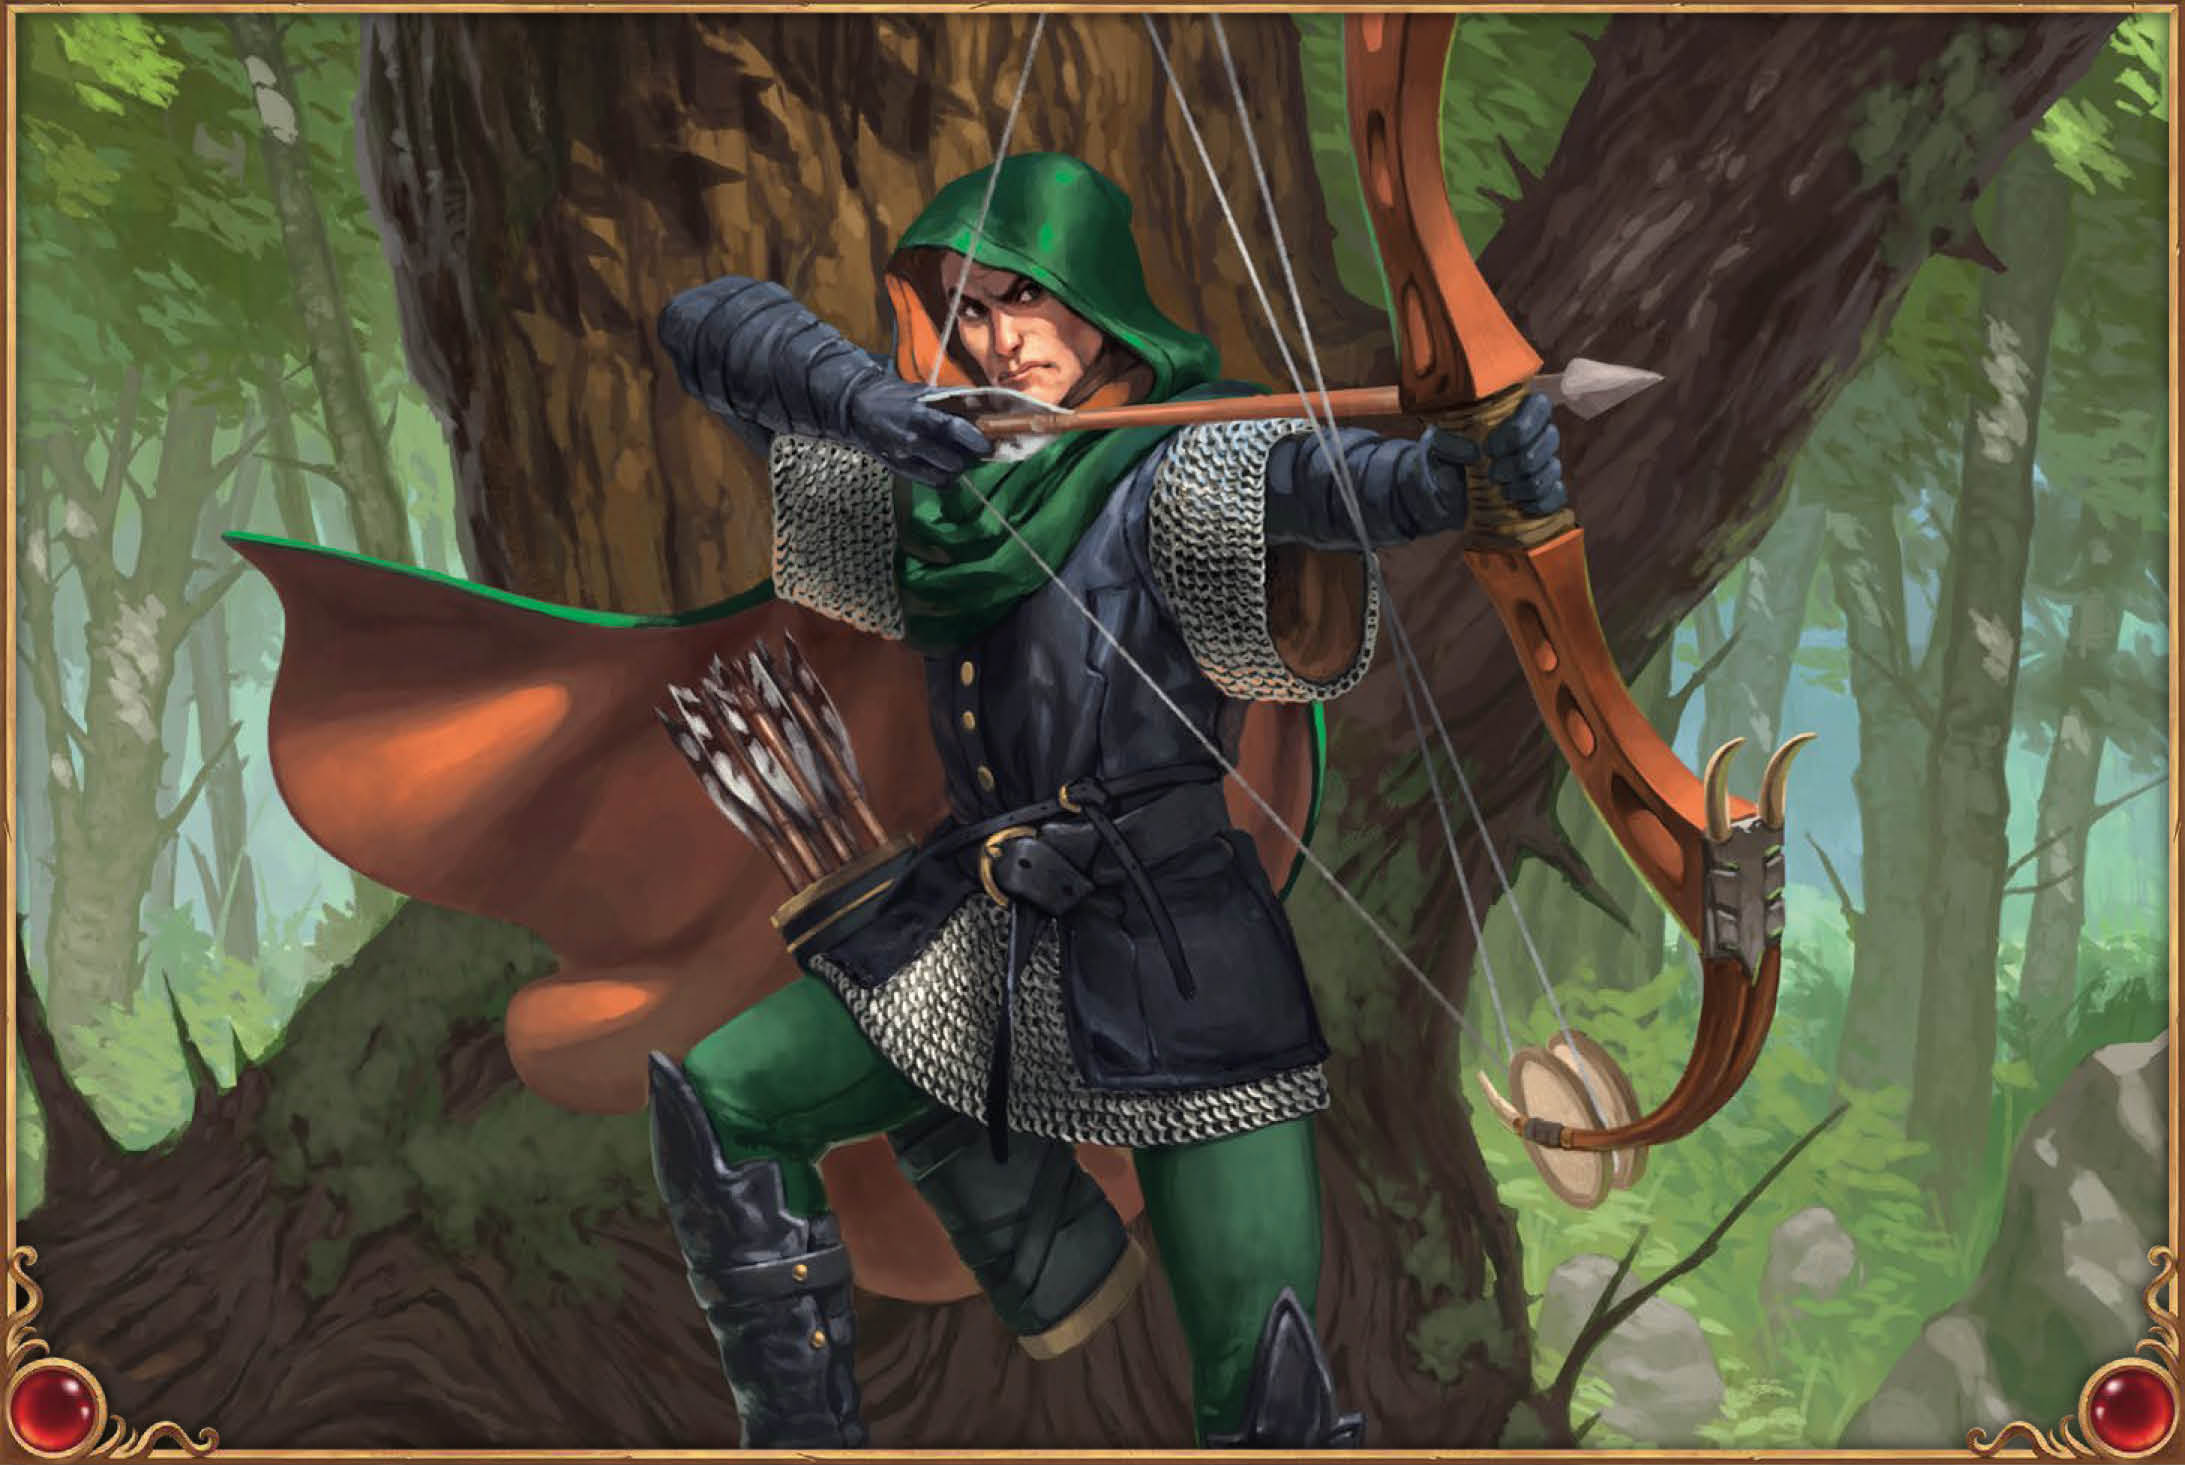
\includegraphics[width=\linewidth, height=\myspace, keepaspectratio]{\art/sharpshooter.jpg}
\end{scaledfigure}

\clearpage

\subsection*{Example}

\begin{multicols*}{2}
\textit{Sandro's Zombies are about to attack Catherine's Griffins.
As Sandro announces the attack, both players now have a chance to modify the attack or defense of their own Unit by playing any number of \includesvg[height=10px]{\svgs/instant.svg} cards that increase an attacking Unit's \includesvg[height=10px]{\svgs/attack.svg} or a defending Unit's \includesvg[height=10px]{\svgs/defense.svg}.}\par
\textit{Sandro decides to play a +1 Attack Card, increasing the Zombies' attack from 2 to 3.
Catherine responds by playing a +1 Defense Card, increasing the Griffins' defense from 0 to 1.
They would both be permitted to play any amount of additional cards in any order, but they decide to stop after playing these cards.}\par

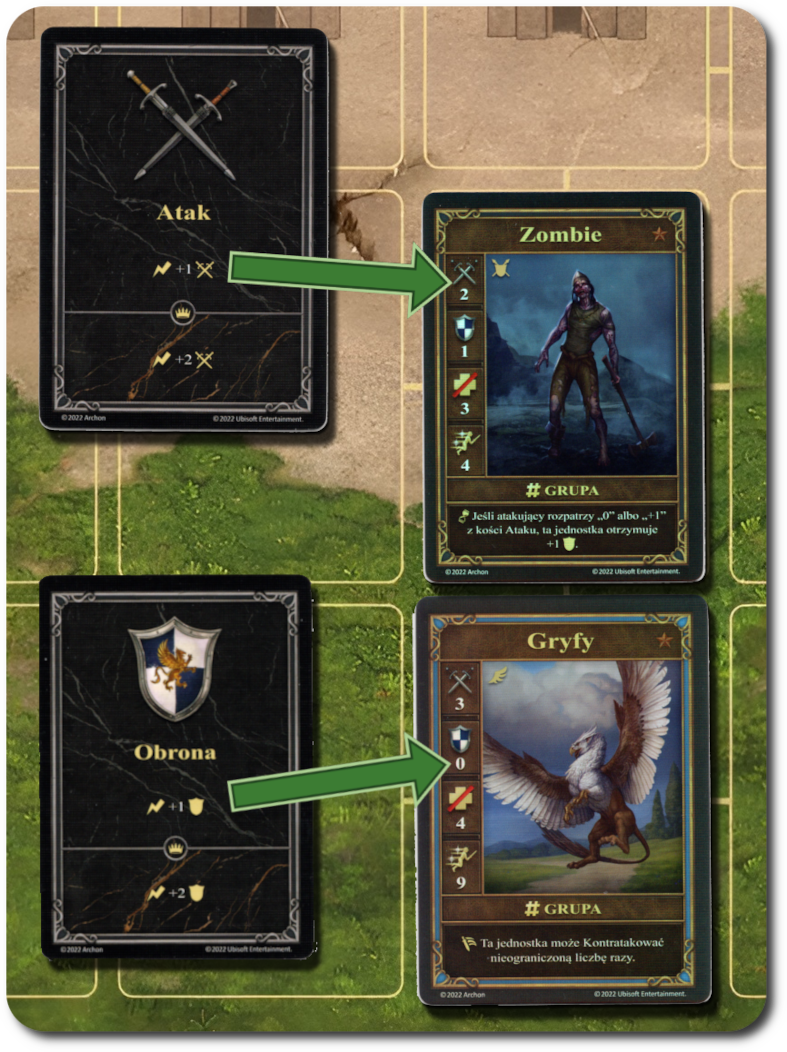
\includegraphics[width=\linewidth]{\examples/zombies_attack_griffins.png}

\textit{After all cards for the attack have been played, the Attack Die is thrown to further modify the amount of damage the attacking Unit deals.
Sandro throws a +1.
This increases the Zombies' attack from 3 to 4, which is then reduced by the Griffins' defense of 1. Therefore, 3 damage \includesvg[height=10px]{\svgs/damage.svg} is placed on the Griffins. Since they have a HP \includesvg[height=10px]{\svgs/health_points.svg} of 4, they are not removed from the Combat.}\par
\textit{The Griffins do not have a black cube on them, therefore they now start a Retaliation Attack.
The cube would now normally be placed on them, however their Special \includesvg[height=10px]{\svgs/unit_retaliate.svg} Ability indicates that they may Retaliate any number of times so the cube is not placed.}\par
\textit{Relatiation Attacks work identically to a normal attack, with the exception that they do not cause another Retaliation Attack.
Therefore, both players are now allowed to modify the statistics of their units again.
The previously played Attack and Defense cards no longer have any effect.}

\vfill

\hspace{-2em}
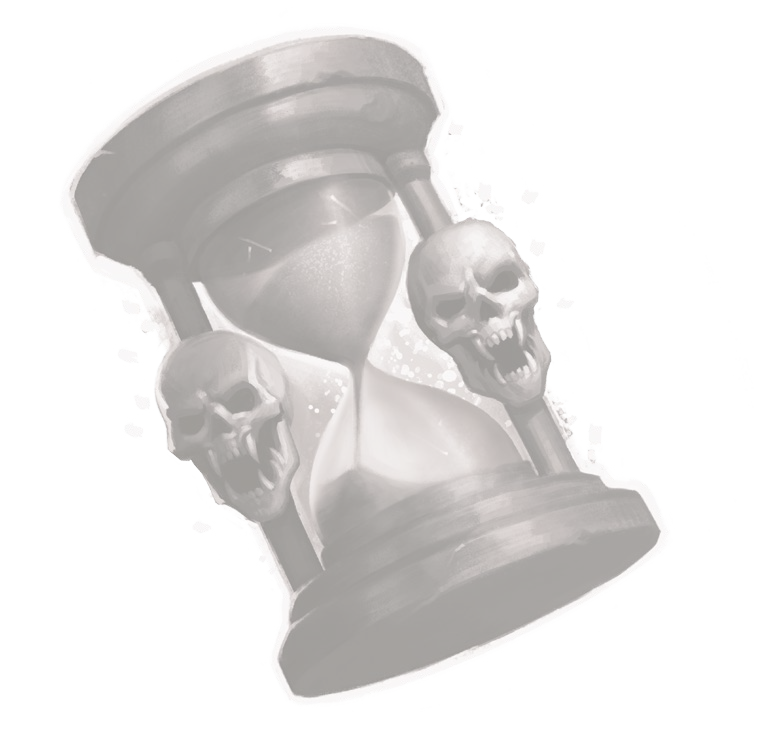
\includegraphics[width=1.4\linewidth]{\art/aging.png}


\end{multicols*}
